\documentclass{beamer}
\makeatletter
\defbeamertemplate*{section page}{mytheme}[1][]{
	\begin{figure}
  \centering
  \begin{minipage}{0.45\textwidth}
	  \centering
    %\raggedright
    \usebeamercolor[fg]{section title}
    \usebeamerfont{section title}
	\insertsectionhead\\[-1ex]
    %\par
    \ifx\insertsubsectionhead\@empty\else%
      \usebeamercolor[fg]{subsection title}%
      \usebeamerfont{subsection title}%
      \insertsubsectionhead
    \fi
\end{minipage}
\begin{minipage}{0.45\textwidth}
	\centering
	\vskip0.5cm
    \ifstrempty{#1}{}{%
		\flushright
		\includegraphics[width=\textwidth]{#1}%
    }
  \end{minipage}
  \end{figure}
  %\par
  %\vspace{\baselineskip}
}
\makeatother

%%% Define a command to include picture in section, 
%%% make section, and revert to old template

\newcommand{\sectionpic}[2]{
   \setbeamertemplate{section page}[mytheme][#2]
   \section{#1}
   \setbeamertemplate{section page}[mytheme]
}





\makeatletter
\setbeamertemplate{footline}{%
\leavevmode
\vbox{\begin{beamercolorbox}[dp=1.25ex,ht=2.75ex]{fg=black}%
  \hspace*{1em}\insertsectionhead%
  \ifx\insertsubsectionhead\@empty\relax\else$\quad\mid\quad$\insertsubsectionhead\fi
  \end{beamercolorbox}%
  }%
}
\makeatother



%\usepackage{pgfpages}
%\setbeameroption{show notes on second screen=right}
%setup images
\usepackage{graphicx}
\graphicspath{{./pics/}}
%equations and vectors
\usepackage[arrowdel]{physics}
\usepackage[normalem]{ulem}
%theme
\usetheme[numbering=counter,progressbar=none,sectionpage=simple]{metropolis}
%references
\usepackage[backend=biber,citestyle=authoryear,bibstyle=numeric,autocite=footnote,firstinits=true]{biblatex}
\DeclareNameAlias{default}{family-given}
\addbibresource{references.bib}
\renewcommand*{\bibfont}{\scriptsize}
\setbeamertemplate{bibliography item}[text]
\renewcommand*{\nameyeardelim}{\addcomma\space}
%theme colors
\definecolor{mGreen}{HTML}{001514} %dark green for titles and frame headings
\definecolor{mBrown}{HTML}{422e24} %dark brown text
\definecolor{mEm}{HTML}{00625d} %light green for emphasis
\definecolor{mBg}{HTML}{E5DDC7} %background tan
\setbeamercolor{normal text}{fg=mBrown,bg=mBg}
\setbeamercolor{example text}{fg=mBrown,bg=mBg}
\setbeamercolor{title separator}{fg=mGreen}
\setbeamercolor{title}{fg=mGreen}
\setbeamercolor{subtitle}{fg=mBrown}
\setbeamercolor{frametitle}{bg=mGreen, fg=mBg}
%custom footnotes
\newcommand{\customfootnotetext}[2]{{
\renewcommand{\thefootnote}{#1}
\footnotetext[0]{#2}}}

\title{Fluxions, Forces, and Fields:}
\subtitle{\small \emph{An overview of the mathematisation of physics in Europe through the modern period}}
\date{\today}
\author{Zella Baig}
%\institute{St. Hilda's College}
\begin{document}
\maketitle
%\section{A Look Back}
  %\begin{frame}{Mathematics in Modern Physics}
	  %\begin{itemize}
		  %\item 'Modern' physics is clearly mathematical:
	  %\end{itemize}
	  %\begin{align*}
		  %\div \va* E &= \frac{\rho}{\epsilon_0} & \div \va* B &= 0\\ 
		 %\curl \va*{E} &=  - \pdv{ \va*B}{t} & \curl \va* B &=  \mu_0\left( \va* J + \epsilon_0 \pdv{\va*E}{t} \right)
	  %\end{align*}
	  %\begin{itemize}
		  %\item Or even more recent:
	  %\end{itemize}
	  %\begin{equation*}
		  %i \hbar \pdv{\ket{\psi}}{t} = \hat H \ket{\psi}
	  %\end{equation*}
  %\end{frame}
  %\begin{frame}{Mathematics in Modern Physics}
      %\frametitle{Mathematics in Modern Physics}
	  %\begin{itemize}
		  %\item But this wasn't always the case
		  %\item The \emph{expectation} (or even requirement) that a physicist be mathematically adept only arose $\sim$ C20 
			  %\note[item]{Mathematics within science is a somewhat recent idea - experiment was key}
		%\item Vector notation had only been around for $\sim$ 50 years!
			%\note[item]{We will discuss vector notation later in fact}
	  %\end{itemize}
  %\end{frame}
  \begin{frame}{Tracing Back}
	\begin{itemize}
		\item Let's take a convenient starting point: Einstein, special relativity, \& aether theory
			\note[item]{No real reason, but more just commonly known as a 'big' event}
		\item Much of the groundwork had been laid by Lorentz, with his \emph{Theory of Corresponding States}{\autocite{specrel}}
		%\only{which generalised length-contraction theory to Maxwell's equations}
	\item Much of the work Lorentz built on was done by George Fitzgerald, who was also influenced greatly by Maxwell
		\note[item]{So we can already begin to draw these links between these (famous) people}
	\end{itemize}
  \end{frame}
  \begin{frame}{Beyond Maxwell}
  	\begin{itemize}
		%\item Maxwell himself adept at maths - 2\textsuperscript{nd} Wrangler
			%\note[item]{Explain what wrangler means}
		\item 'Mentored' by William Thomson{\autocite{newchart}}  (later Lord Kelvin)\ldots
			\note[item]{explain this was a professional/guiding relationship}
			\only{who was a major figure in shaping physics (or natural philosophy) in C19} 
		\item Physics in Thomson's day had been centred around energy (and thus dynamics)\ldots
			\note[item]{Mention how we will analyse why it was dynamics which dominated energy}
		\item\ldots Which followed from continental development furthered by figures such as Lagrange and Laplace\ldots
		\item \ldots Who worked using methods derived from Newton's work on celestial motion
			\note[item]{Mention how we can now see there's a clear line of succession, and we'll be looking at how each figure influenced the next}
  	\end{itemize}
  \end{frame}
  %\begin{frame}{Not Just Mathematics}
	  %Of course, there are other overarching themes as well:
	  %\begin{itemize}
		  %\item Baconian ideals,
			  %\note[item]{Explain what baconianism is - empiricism, collaboration, etc. Science was investigated. This leads on well to the next point}
		  %\item Collaborative bodies such as the Royal Institute,
		  %\item \onslide And (again from Newton) \emph{\color{mEm}hypotheses non fingo}\textsuperscript{i}
	  %\end{itemize}
	  %{\only\customfootnotetext{i}{To be discussed later on}}
  %\end{frame}
%\section{Pre-Newtonianism}%
%\begin{frame}{Natural Philosophy Pre Early Modern Period}
	%\begin{itemize}
		%\item 'Physics' (or Natural Philosophy) focused largely on astronomy
			%\begin{itemize}
				%\item[--] the ``noblest of all'' mathematical disciplines\autocite{clavius}
			%\end{itemize}
		%\item Aristotle's views regarding 'empiricism' \& 'perfection' largely dominant
			%\note[item]{Discuss how this doesn't imply stagnation, but merely shaped how the world was viewed as well as the approach to science}
		%\item Mathematics had been largely distinct, again due to ancient influences
			%\note[item]{It still was studied, and it was rigourous, but it wasn't a science and was almost a 'plaything'}
		%\item First major (relevant) shift comes with Bacon \& his \emph{Novum Organum}{\autocite{novorg}} {\color{mEm}- the birth of the scientific method?}
	%\end{itemize}
%\end{frame}
  \sectionpic{The Birth of an Era: \\Isaac Newton\\\scriptsize{(1643-1727)}}{newton}
\begin{frame}{Newtonian Mathematical Ideals}
	%\begin{figure}[h]
		%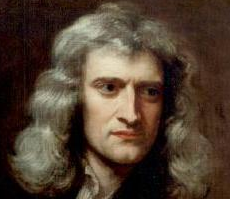
\includegraphics[scale=0.2]{newt}
	%\end{figure}
	\begin{itemize}
		\item \onslide Saw God as mathematical, with a fondness for geometry
			\note[item]{Mention how in his work he would often discuss god, and the ancients}
			\note[item]{also bring up how his physical work is but a portion of his alchemy and other work}
		\item Fluxions \& Fluents\textsuperscript{i}
		\item Clashes with Cartesianism\autocite{westfall}
			\note[item]{One major reason for this was the concept of force at a distance}
		%\item Sought 'elegance' in mathematics{ \autocite{westfall}}
			%\note[item]{As well as being haughty, he was also a very petty man - bring up removing 'esteemed' to 'mr'}
	\end{itemize}
	\customfootnotetext{i}{For reading on notational impact, see: \cite{guiccardinidevelopment,dotage,boyercalc}}
\end{frame}
\begin{frame}{Experimental Philosophy}
	\begin{itemize}
		\item The method of {\color{mEm}{resolution}} \& {\color{mEm}{composition:}}
			\note[item]{Mention how sometimes it appears as if Newton himself didn't know what he meant; conflicting uses}
			\begin{enumerate}
				\item Observe and ``come to the general properties of things''{\only\autocite{newtonprinc}}
				\item Assume said properties and describe further phenomena
			\end{enumerate}
		\item {\color{mEm}{Hypotheses non fingo}}\autocite{principia} - ignorance is acceptable!
			%\begin{itemize}
				%\item[--] Now able to make predictions using mathematical tools - without worrying about cause 
			%\end{itemize}
		\item Nature able to be quantised (e.g. fluxional calculus \& Halley's Comet)
			\note[item]{Discuss in detail - getting measurements from Flamsteed, the royal astronomer, and applying etc}
			\begin{itemize}
				\item[--] Concept of forces at a distance
			\end{itemize}
		%\item Important to note the ramifications of geometric arguments
			%\note[item]{Religious backing, make his work iron clad as to prevent arguments against it}
	\end{itemize}
\end{frame}
%\begin{frame}{Gottfried Leibniz (1646-1716)}
	%\begin{itemize}
		%\item Who discovered calculus first?
			%\note[item]{Newton discovered first, as he claims, but leibniz published first. Newton quarrels as usual}
		%\item Leibnizian calculus seen as inelegant
			%\note[item]{Again newton preferring geometry, or perhaps to cover up that he had published later as he was perfecting it}
		%\item Some literature suggests Newton's notation might have impeded British science
			%\note[item]{Discuss fluxions (which are adding eg a small dt term), and fluents which are both integrals and derivatives of functions of time. Mention sloppy notation usage}
			%\begin{itemize}
				%\item[--] \emph{The Development of Newtonian Calculus} { \autocite{guiccardinidevelopment}}
				%\item[--] \emph{Dot-Age}{ \autocite{dotage}}
				%\item[--]\emph{The History of Calculus} {\autocite{boyercalc}}
					%\note[item]{Discuss how this isn't likely the major factor, as the next head of the royal society was very anti newton}
			%\end{itemize}
		%\item Regardless, we are interested in the {\color{mEm}physical} influences of calculus
			%\note[item]{Newton's calculus more influential simply for the scientific ramifications - his philosophy and the discovery of Halley's comet}
	%\end{itemize}
%\end{frame}
%\section{The Dynamical Age: Continental Physics}%
  \sectionpic{The Dynamical Age: Pierre-Simon Laplace\\\scriptsize{(1749-1827)}}{laplace}
%\begin{frame}{Putting Calculus to Use}
	%\begin{itemize}
		%\item Euler, Clairaut, and others applied Newton's experimental philosophy\autocite{shapiro} to various problems, gradually verifying several with observations
			%\begin{itemize}
				%\item[--] Clairaut's work on the three-body problem particularly important
					%\note[item]{This showed that newton's work really was quite important - it had allowed for major work towards the problem which had stumped many other mathematicians. Lent credit to newton}
			%\end{itemize}
		%\item Development of Lagrangian mechanics \& applications to further contexts (such as the motion of sound)
	%\end{itemize}
%\end{frame}
\begin{frame}{Laplacian Physics}
\begin{itemize}
	\item The rise of French scientific dominance
		\note[item]{Discuss napoleons upbringing - had laplace as a teacher, was fond of mathematics}
	\item Physics spearheaded by Laplace (1749-1827) in early C19, who took an ''astronomical view of nature''{ \autocite{merz}}
	\item Prevalence of central-force based models, for even minute scales{ \autocite{foxl}}
		\note[item]{these had traditionally been the bread and butter of newtonian calculus}
	\item Competitions set-up with e.g. the Society of Arcueil to promote mathematical collaboration
		\note[item]{Allowed for great development of ideas internationally}
	\item Development of light, heat, and electromagnetic theory with various contestants (e.g. Fourier) - via Laplacian methods
\end{itemize}
\end{frame}
%\section{Energy Physics}%
  \sectionpic{Heating Up:\\ William Thomson\\\scriptsize{(1824-1907)}}{kv}
\begin{frame}{Thomson \& Energy}
	\begin{itemize}
		\item Ideas of \emph{vis-viva} around since Leibniz, \emph{caloric} furthered by e.g. Carnot in early C19
			\note[item]{Energy ideas were floating around - it being created, being a fluid, etc}
		\item Natural philosophy shifted towards a focus on (conservation of) energy - in particular heat{ \autocite{newchart}}
			\note[item]{Many reasons for this - perhaps discuss steam engines, practical applications. Baconiamism - applications of science to improving lives}
			%\begin{itemize}
				%\item[--] Appealing due to {\color{mEm}all} physics being related (perhaps even dynamically!)
			%\end{itemize}
		\item Thomson follows Newtonian ideals - refusing to assign hypotheses
		\item There exist ``absolute numerical relations'' between heat and power{\only \autocite{thomdynam}}
			\note[item]{Thomson knew there was something relating heat and energy, investigated it}
	\end{itemize}
\end{frame}
%\begin{frame}{Thomson \& Tait}
%\begin{itemize}
	%\item Together, they publish \emph{Treatise on Natural Philosophy}\autocite{treatise}: the first high-level {\color{mEm}mathematically-inclined} physics textbook\textsuperscript{iii}, as well as a synthesis of their work on energy 
	%\item Intended to ``give in three moderate volumes a far more complete course of Physics, Experimental and Mathematical, than exists''{ \autocite{taitletter}}
%\end{itemize}
%\customfootnotetext{iii}{In fact, 'energy' as a concept was not taught much \emph{at all}}
%\end{frame}
  \sectionpic{Models and Mathematics:\\James Clerk Maxwell\\\scriptsize{(1831-1879)}}{gg}
%\section{James Maxwell (1831-1879)}%
%\begin{frame}{Maxwell \& Thomson}
%\begin{itemize}
	%\item Both mathematically inclined Scottish physicists (contrasting to e.g. Faraday) \autocite{Gooding1985}
	%\item Thomson guided Maxwell's intellectual pursuits both directly and indirectly:
		%\note[item]{Thomson busy with other pursuits, told to read on faraday as thomson (and the world) recognised his brilliance}
		%\note[item]{faraday the opposite of a mathematician - almost all practical work, but amazing experimenter; give brief overview}
		%\begin{itemize}
			%\item[--] ``The discussion of the various forms of energy \ldots constitutes the whole of physical science''{\autocite{matter}}
				%\note[item]{Quote from several years later but you can see how thomson influenced maxwell}
		%\end{itemize}
	%\item On electromagnetism, pondered the nature of the 'store' of energy, e.g. in his \emph{Dynamical Theory}{ \autocite{maxdynamicaltheory}}
%\end{itemize}
%\end{frame}
\begin{frame}{The Birth of Electromagnetism}
	\begin{itemize}
		\item Faraday had done groundbreaking work on electromagnetism, but almost entirely qualitative
		\item Maxwell reticent to attribute any physical cause; \emph{Faraday's Lines}{\only \autocite{maxfaradaylines}} makes no claim of physicality
			\note[item]{Instead claims to be a mathematical model which he uses to develop Faraday's work}
		\item \emph{Dynamical Theory}\autocite{maxdynamicaltheory} made little note of aether as it was mathematically unnecessary
			\note[item]{This was interesting given how much of a headache aether theory had caused EM models}
		\item \emph{Physical Lines}{ \autocite{maxphysicallines}} - first postulates light being electromagnetic, as well as displacement current
		%\item Work culminates in his \emph{Treatise}{ \autocite{maxtreatise}}
	\end{itemize}
%\footnotetext[2]{He also first introduced the notion of a 'field'}
\end{frame}
%\begin{frame}{Vortex Model}
	%\begin{figure}[h!]
	%\begin{center}
		%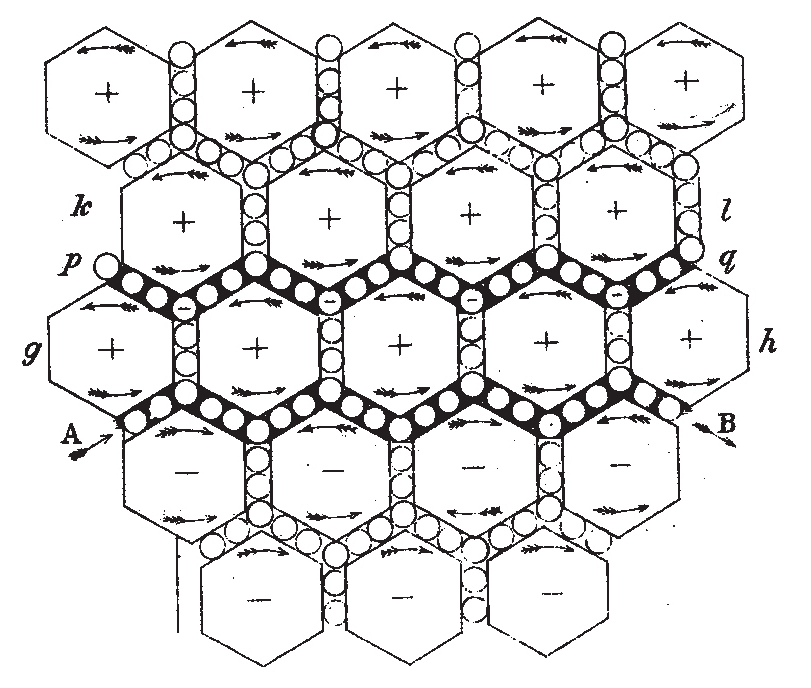
\includegraphics[width=0.7\textwidth]{vortex}
	%\end{center}
	%\caption{Maxwell's 'vortex \& idle-wheel' model, in \emph{Physical Lines} }
	%\end{figure}
	%\note[item]<1>{Describe the motion of the wheels and current particles; explain how it led to the curl dependence}
%\end{frame}

\begin{frame}{Maxwell \& Vectors}
	\begin{itemize}
		%\item Greatly develops vector calculus out of necessity for his mechanical models
		\item Greatly develops \sout{vector} calculus out of necessity for his mechanical models {\color{mEm}- Maxwell didn't have vector notation at his disposal!}
		\item Modern formulation only introduced in 1884, by Heavyside{ \autocite{heavyside}}
			%\begin{itemize}
				%\item[--] From 20 equations to 4
					%\note[item]{Discuss how there were various other parameters each representing components of fields along certain axes}
					%\note[item]{Also mention how this led to conceptual complexity - dealing with so many interconnected equations}
			%\end{itemize}
		\item Vector notation itself only introduced in 1843, by Hamilton \autocite{vecanal}
			%, with a 'recognisable' form appearing later that century via Clifford, Gibbs, and Heavyside{ \autocite{vecanal}}
			\note[item]{Discuss how this was brought about with textbook usage by Clifford and Gibbs mainly, when lecturing in the US. Heavyside was mainly consolidating Maxwell's work}
	\end{itemize}
\end{frame}
  \sectionpic{Transformations \& Time:\\Henri Poincaré\\\scriptsize{(1854-1912)}}{ponc}
\begin{frame}{The First Cracks}
\begin{itemize}
	\item Following Maxwell's work, electromagnetism became dominant{ \autocite{maxwellians}}
		\note[item]{Dominant in the sense it led to an explosion of work around electromagnetism, light, and energy.}
	\item  The nature of the aether was hotly debated
		\note[item]{Discuss michelson morley experiment and conflicting results - stokes' dragging hypotheses, fizeaus water experiment etc.}
	\item Lorentz develops ideas of 'local time' \& 'corresponding states' (co-ordinate transforms - \emph{but only of EM waves}\autocite{brownspec})
		%\begin{itemize}
			%\item[--] A {\color{mEm} \bf purely} mathematical construction{ \autocite{brownspec}}
				%\note[item]{Stress this point - Lorentz was seemingly not aware of the physical connotations; had merely shown that this was a hypothesis that could work. Also had funnily enough made a factor of 2 error in his work}
		%\end{itemize}
\end{itemize}
%\only\customfootnotetext{iv}{In fact, Newton's initial work necessitated a vacuum in space}
%\footnotetext[3]{Largely by the \emph{Maxwellians:} Lodge, Fitzgerald, Hertz, and others}
\end{frame}
\begin{frame}{Developing Physicality}
	\begin{itemize}
		%\item Able to infer physicality of Lorentz' transformations{ \autocite{darrigol}}
		\item Develops theory to be (functionally) identical to modern Lorentz transformations\autocite{darrigol}
		\item Willing to ignore aether hypotheses, as mathematically unnecessary{ \autocite{poincare}}
			\begin{itemize}
				\item[--] Unwilling to fully commit to ideas: ``Of hypotheses there is never lack''{ \autocite{fond}}
					\note[item]{He may also have been unwilling to let go of the idea of aether theory, or alternatively he may not have actually grasped the ramifications of what this implied for aether theory}
			\end{itemize}
		\item Einstein would soon go on to have his \emph{annus mirabilis} and completely shift away from aether theory
	\end{itemize}
\end{frame}
\section{Conclusion}%
\begin{frame}{To Sum Up\ldots}
	\begin{itemize}
		\item Initial shift with Newton's development of \emph{experimental philosophy} and quantisation of nature
		\item  Development of continental force-based physics 
		\item  Shift towards disciplinary rigour with Thomson and others
		\item  Maxwellian development of electromagnetic theory
		\item The final steps away from the aether - after thousands of years
			\note[item]{discuss how we have had a massive shift in just the period of a few hundred years - can link it with the explosive rate of human growth as well. Discuss how it has led to so much advance in science and mathematics, as the lines between the two are blurred.}
	\end{itemize}
\end{frame}
\section{\color{mGreen}Thank You}%
\section{References}%
\begin{frame}[allowframebreaks]
	\nocite{*}
	\printbibliography[heading=none]
\end{frame}
\end{document}
